\documentclass[twoside]{book}

% Packages required by doxygen
\usepackage{fixltx2e}
\usepackage{calc}
\usepackage{doxygen}
\usepackage[export]{adjustbox} % also loads graphicx
\usepackage{graphicx}
\usepackage[utf8]{inputenc}
\usepackage{makeidx}
\usepackage{multicol}
\usepackage{multirow}
\PassOptionsToPackage{warn}{textcomp}
\usepackage{textcomp}
\usepackage[nointegrals]{wasysym}
\usepackage[table]{xcolor}

% Font selection
\usepackage[T1]{fontenc}
\usepackage[scaled=.90]{helvet}
\usepackage{courier}
\usepackage{amssymb}
\usepackage{sectsty}
\renewcommand{\familydefault}{\sfdefault}
\allsectionsfont{%
  \fontseries{bc}\selectfont%
  \color{darkgray}%
}
\renewcommand{\DoxyLabelFont}{%
  \fontseries{bc}\selectfont%
  \color{darkgray}%
}
\newcommand{\+}{\discretionary{\mbox{\scriptsize$\hookleftarrow$}}{}{}}

% Page & text layout
\usepackage{geometry}
\geometry{%
  a4paper,%
  top=2.5cm,%
  bottom=2.5cm,%
  left=2.5cm,%
  right=2.5cm%
}
\tolerance=750
\hfuzz=15pt
\hbadness=750
\setlength{\emergencystretch}{15pt}
\setlength{\parindent}{0cm}
\setlength{\parskip}{3ex plus 2ex minus 2ex}
\makeatletter
\renewcommand{\paragraph}{%
  \@startsection{paragraph}{4}{0ex}{-1.0ex}{1.0ex}{%
    \normalfont\normalsize\bfseries\SS@parafont%
  }%
}
\renewcommand{\subparagraph}{%
  \@startsection{subparagraph}{5}{0ex}{-1.0ex}{1.0ex}{%
    \normalfont\normalsize\bfseries\SS@subparafont%
  }%
}
\makeatother

% Headers & footers
\usepackage{fancyhdr}
\pagestyle{fancyplain}
\fancyhead[LE]{\fancyplain{}{\bfseries\thepage}}
\fancyhead[CE]{\fancyplain{}{}}
\fancyhead[RE]{\fancyplain{}{\bfseries\leftmark}}
\fancyhead[LO]{\fancyplain{}{\bfseries\rightmark}}
\fancyhead[CO]{\fancyplain{}{}}
\fancyhead[RO]{\fancyplain{}{\bfseries\thepage}}
\fancyfoot[LE]{\fancyplain{}{}}
\fancyfoot[CE]{\fancyplain{}{}}
\fancyfoot[RE]{\fancyplain{}{\bfseries\scriptsize Generated by Doxygen }}
\fancyfoot[LO]{\fancyplain{}{\bfseries\scriptsize Generated by Doxygen }}
\fancyfoot[CO]{\fancyplain{}{}}
\fancyfoot[RO]{\fancyplain{}{}}
\renewcommand{\footrulewidth}{0.4pt}
\renewcommand{\chaptermark}[1]{%
  \markboth{#1}{}%
}
\renewcommand{\sectionmark}[1]{%
  \markright{\thesection\ #1}%
}

% Indices & bibliography
\usepackage{natbib}
\usepackage[titles]{tocloft}
\setcounter{tocdepth}{3}
\setcounter{secnumdepth}{5}
\makeindex

% Hyperlinks (required, but should be loaded last)
\usepackage{ifpdf}
\ifpdf
  \usepackage[pdftex,pagebackref=true]{hyperref}
\else
  \usepackage[ps2pdf,pagebackref=true]{hyperref}
\fi
\hypersetup{%
  colorlinks=true,%
  linkcolor=blue,%
  citecolor=blue,%
  unicode%
}

% Custom commands
\newcommand{\clearemptydoublepage}{%
  \newpage{\pagestyle{empty}\cleardoublepage}%
}

\usepackage{caption}
\captionsetup{labelsep=space,justification=centering,font={bf},singlelinecheck=off,skip=4pt,position=top}

%===== C O N T E N T S =====

\begin{document}

% Titlepage & ToC
\hypersetup{pageanchor=false,
             bookmarksnumbered=true,
             pdfencoding=unicode
            }
\pagenumbering{alph}
\begin{titlepage}
\vspace*{7cm}
\begin{center}%
{\Large the forsaken playground \\[1ex]\large 1 }\\
\vspace*{1cm}
{\large Generated by Doxygen 1.8.13}\\
\end{center}
\end{titlepage}
\clearemptydoublepage
\pagenumbering{roman}
\tableofcontents
\clearemptydoublepage
\pagenumbering{arabic}
\hypersetup{pageanchor=true}

%--- Begin generated contents ---
\chapter{Data Structure Index}
\section{Data Structures}
Here are the data structures with brief descriptions\+:\begin{DoxyCompactList}
\item\contentsline{section}{\hyperlink{structobj}{obj} \\*Struct for obj }{\pageref{structobj}}{}
\item\contentsline{section}{\hyperlink{structObjet}{Objet} }{\pageref{structObjet}}{}
\item\contentsline{section}{\hyperlink{structvie}{vie} \\*Struct for vie }{\pageref{structvie}}{}
\end{DoxyCompactList}

\chapter{File Index}
\section{File List}
Here is a list of all documented files with brief descriptions\+:\begin{DoxyCompactList}
\item\contentsline{section}{\hyperlink{main_8c}{main.\+c} \\*Testing Program }{\pageref{main_8c}}{}
\item\contentsline{section}{\hyperlink{temps_8c}{temps.\+c} }{\pageref{temps_8c}}{}
\item\contentsline{section}{\hyperlink{temps_8h}{temps.\+h} }{\pageref{temps_8h}}{}
\end{DoxyCompactList}

\chapter{Data Structure Documentation}
\hypertarget{structtemps}{}\section{temps Struct Reference}
\label{structtemps}\index{temps@{temps}}


struct for time  




{\ttfamily \#include $<$temps.\+h$>$}

\subsection*{Data Fields}
\begin{DoxyCompactItemize}
\item 
int \hyperlink{structtemps_a2011835f5e7a49a1233eda77a44dd2e5}{heur1}
\item 
int \hyperlink{structtemps_a54b7d1185a09a8fb91dba7e6509bcd15}{heur2}
\item 
int \hyperlink{structtemps_a400cb69ff8af9b43eb6abab78fa0161c}{minute1}
\item 
int \hyperlink{structtemps_a2414045fced292cf676b7fd59ec9181c}{minute2}
\item 
int \hyperlink{structtemps_a5c5612243cfd9e4e379f5c3d8b60fa01}{seconde1}
\item 
int \hyperlink{structtemps_a7fcb75d6c82d79b83d53c2312e2b86a0}{seconde2}
\item 
S\+D\+L\+\_\+\+Surface $\ast$ \hyperlink{structtemps_aab50e212cfeca5de8ced5c501f0120ba}{temp}
\item 
S\+D\+L\+\_\+\+Rect \hyperlink{structtemps_a77d09ab78c81ed3951ff41e1974cc14d}{position\+\_\+temp}
\item 
T\+T\+F\+\_\+\+Font $\ast$ \hyperlink{structtemps_a5496aa7ef92a402878dfa83dc44cb570}{police}
\item 
int \hyperlink{structtemps_ab07c63dc7591472ca0214e52ff4cb014}{tempactuel}
\item 
int \hyperlink{structtemps_a94454b9ce545c311e78f31f7add21952}{tempprecedent}
\item 
char \hyperlink{structtemps_a7887aa391bcc303452f3b173e5ba89ce}{chaine} \mbox{[}20\mbox{]}
\end{DoxyCompactItemize}


\subsection{Detailed Description}
struct for time 

\subsection{Field Documentation}
\mbox{\Hypertarget{structtemps_a7887aa391bcc303452f3b173e5ba89ce}\label{structtemps_a7887aa391bcc303452f3b173e5ba89ce}} 
\index{temps@{temps}!chaine@{chaine}}
\index{chaine@{chaine}!temps@{temps}}
\subsubsection{\texorpdfstring{chaine}{chaine}}
{\footnotesize\ttfamily char temps\+::chaine\mbox{[}20\mbox{]}}

char \mbox{\Hypertarget{structtemps_a2011835f5e7a49a1233eda77a44dd2e5}\label{structtemps_a2011835f5e7a49a1233eda77a44dd2e5}} 
\index{temps@{temps}!heur1@{heur1}}
\index{heur1@{heur1}!temps@{temps}}
\subsubsection{\texorpdfstring{heur1}{heur1}}
{\footnotesize\ttfamily int temps\+::heur1}

integer \mbox{\Hypertarget{structtemps_a54b7d1185a09a8fb91dba7e6509bcd15}\label{structtemps_a54b7d1185a09a8fb91dba7e6509bcd15}} 
\index{temps@{temps}!heur2@{heur2}}
\index{heur2@{heur2}!temps@{temps}}
\subsubsection{\texorpdfstring{heur2}{heur2}}
{\footnotesize\ttfamily int temps\+::heur2}

integer \mbox{\Hypertarget{structtemps_a400cb69ff8af9b43eb6abab78fa0161c}\label{structtemps_a400cb69ff8af9b43eb6abab78fa0161c}} 
\index{temps@{temps}!minute1@{minute1}}
\index{minute1@{minute1}!temps@{temps}}
\subsubsection{\texorpdfstring{minute1}{minute1}}
{\footnotesize\ttfamily int temps\+::minute1}

integer \mbox{\Hypertarget{structtemps_a2414045fced292cf676b7fd59ec9181c}\label{structtemps_a2414045fced292cf676b7fd59ec9181c}} 
\index{temps@{temps}!minute2@{minute2}}
\index{minute2@{minute2}!temps@{temps}}
\subsubsection{\texorpdfstring{minute2}{minute2}}
{\footnotesize\ttfamily int temps\+::minute2}

integer \mbox{\Hypertarget{structtemps_a5496aa7ef92a402878dfa83dc44cb570}\label{structtemps_a5496aa7ef92a402878dfa83dc44cb570}} 
\index{temps@{temps}!police@{police}}
\index{police@{police}!temps@{temps}}
\subsubsection{\texorpdfstring{police}{police}}
{\footnotesize\ttfamily T\+T\+F\+\_\+\+Font$\ast$ temps\+::police}

police \mbox{\Hypertarget{structtemps_a77d09ab78c81ed3951ff41e1974cc14d}\label{structtemps_a77d09ab78c81ed3951ff41e1974cc14d}} 
\index{temps@{temps}!position\+\_\+temp@{position\+\_\+temp}}
\index{position\+\_\+temp@{position\+\_\+temp}!temps@{temps}}
\subsubsection{\texorpdfstring{position\+\_\+temp}{position\_temp}}
{\footnotesize\ttfamily S\+D\+L\+\_\+\+Rect temps\+::position\+\_\+temp}

position du temps dans l\textquotesingle{}ecran. \mbox{\Hypertarget{structtemps_a5c5612243cfd9e4e379f5c3d8b60fa01}\label{structtemps_a5c5612243cfd9e4e379f5c3d8b60fa01}} 
\index{temps@{temps}!seconde1@{seconde1}}
\index{seconde1@{seconde1}!temps@{temps}}
\subsubsection{\texorpdfstring{seconde1}{seconde1}}
{\footnotesize\ttfamily int temps\+::seconde1}

integer \mbox{\Hypertarget{structtemps_a7fcb75d6c82d79b83d53c2312e2b86a0}\label{structtemps_a7fcb75d6c82d79b83d53c2312e2b86a0}} 
\index{temps@{temps}!seconde2@{seconde2}}
\index{seconde2@{seconde2}!temps@{temps}}
\subsubsection{\texorpdfstring{seconde2}{seconde2}}
{\footnotesize\ttfamily int temps\+::seconde2}

integer \mbox{\Hypertarget{structtemps_aab50e212cfeca5de8ced5c501f0120ba}\label{structtemps_aab50e212cfeca5de8ced5c501f0120ba}} 
\index{temps@{temps}!temp@{temp}}
\index{temp@{temp}!temps@{temps}}
\subsubsection{\texorpdfstring{temp}{temp}}
{\footnotesize\ttfamily S\+D\+L\+\_\+\+Surface$\ast$ temps\+::temp}

surface \mbox{\Hypertarget{structtemps_ab07c63dc7591472ca0214e52ff4cb014}\label{structtemps_ab07c63dc7591472ca0214e52ff4cb014}} 
\index{temps@{temps}!tempactuel@{tempactuel}}
\index{tempactuel@{tempactuel}!temps@{temps}}
\subsubsection{\texorpdfstring{tempactuel}{tempactuel}}
{\footnotesize\ttfamily int temps\+::tempactuel}

integer \mbox{\Hypertarget{structtemps_a94454b9ce545c311e78f31f7add21952}\label{structtemps_a94454b9ce545c311e78f31f7add21952}} 
\index{temps@{temps}!tempprecedent@{tempprecedent}}
\index{tempprecedent@{tempprecedent}!temps@{temps}}
\subsubsection{\texorpdfstring{tempprecedent}{tempprecedent}}
{\footnotesize\ttfamily int temps\+::tempprecedent}

integer 

The documentation for this struct was generated from the following file\+:\begin{DoxyCompactItemize}
\item 
\hyperlink{temps_8h}{temps.\+h}\end{DoxyCompactItemize}

\chapter{File Documentation}
\hypertarget{main_8c}{}\section{main.\+c File Reference}
\label{main_8c}\index{main.\+c@{main.\+c}}


Testing Program.  


{\ttfamily \#include $<$stdio.\+h$>$}\newline
{\ttfamily \#include $<$stdlib.\+h$>$}\newline
{\ttfamily \#include $<$S\+D\+L/\+S\+D\+L.\+h$>$}\newline
{\ttfamily \#include $<$math.\+h$>$}\newline
{\ttfamily \#include $<$time.\+h$>$}\newline
{\ttfamily \#include $<$S\+D\+L/\+S\+D\+L\+\_\+image.\+h$>$}\newline
{\ttfamily \#include $<$S\+D\+L/\+S\+D\+L\+\_\+mixer.\+h$>$}\newline
{\ttfamily \#include $<$S\+D\+L/\+S\+D\+L\+\_\+ttf.\+h$>$}\newline
{\ttfamily \#include $<$string.\+h$>$}\newline
{\ttfamily \#include \char`\"{}temps.\+h\char`\"{}}\newline
Include dependency graph for main.\+c\+:
\nopagebreak
\begin{figure}[H]
\begin{center}
\leavevmode
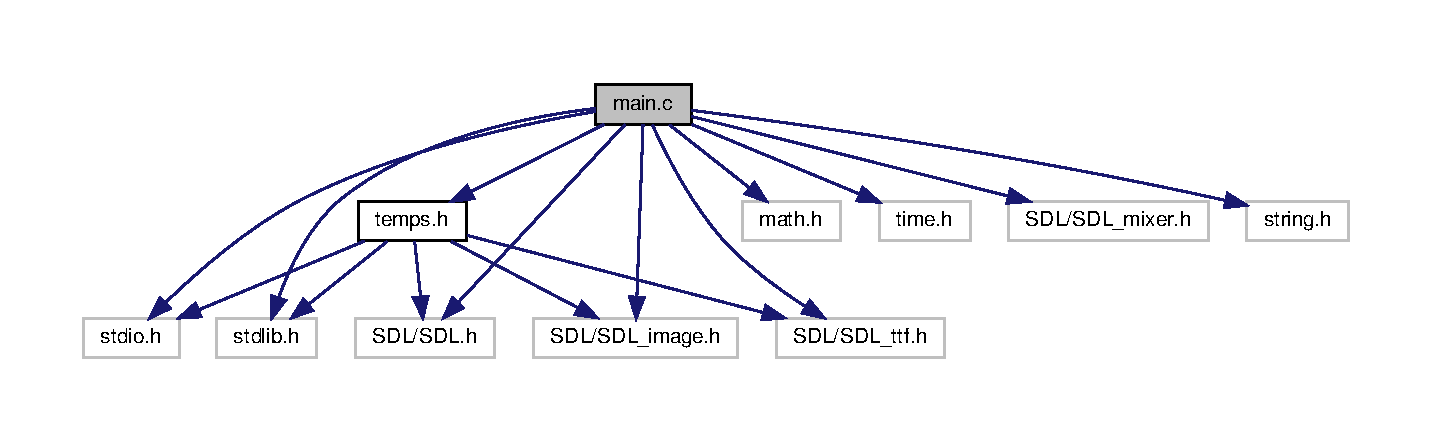
\includegraphics[width=350pt]{main_8c__incl}
\end{center}
\end{figure}
\subsection*{Functions}
\begin{DoxyCompactItemize}
\item 
\mbox{\Hypertarget{main_8c_ae66f6b31b5ad750f1fe042a706a4e3d4}\label{main_8c_ae66f6b31b5ad750f1fe042a706a4e3d4}} 
int {\bfseries main} ()
\end{DoxyCompactItemize}


\subsection{Detailed Description}
Testing Program. 

\begin{DoxyAuthor}{Author}
otail marzouk 
\end{DoxyAuthor}
\begin{DoxyVersion}{Version}
0.\+1 
\end{DoxyVersion}
\begin{DoxyDate}{Date}
mai 07, 2019
\end{DoxyDate}
Testing program for time 
\hypertarget{temps_8c}{}\section{temps.\+c File Reference}
\label{temps_8c}\index{temps.\+c@{temps.\+c}}
{\ttfamily \#include $<$stdio.\+h$>$}\newline
{\ttfamily \#include $<$stdlib.\+h$>$}\newline
{\ttfamily \#include $<$S\+D\+L/\+S\+D\+L.\+h$>$}\newline
{\ttfamily \#include $<$math.\+h$>$}\newline
{\ttfamily \#include $<$time.\+h$>$}\newline
{\ttfamily \#include $<$S\+D\+L/\+S\+D\+L\+\_\+image.\+h$>$}\newline
{\ttfamily \#include $<$S\+D\+L/\+S\+D\+L\+\_\+mixer.\+h$>$}\newline
{\ttfamily \#include $<$S\+D\+L/\+S\+D\+L\+\_\+ttf.\+h$>$}\newline
{\ttfamily \#include $<$string.\+h$>$}\newline
{\ttfamily \#include \char`\"{}temps.\+h\char`\"{}}\newline
Include dependency graph for temps.\+c\+:
\nopagebreak
\begin{figure}[H]
\begin{center}
\leavevmode
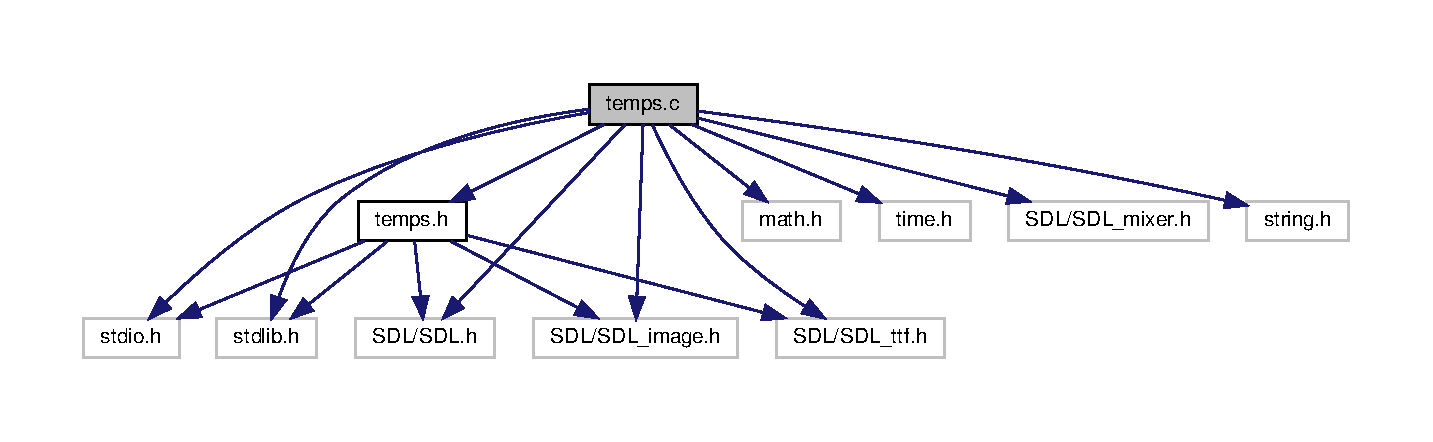
\includegraphics[width=350pt]{temps_8c__incl}
\end{center}
\end{figure}
\subsection*{Functions}
\begin{DoxyCompactItemize}
\item 
\hyperlink{structtemps}{temps} \hyperlink{temps_8c_a8e74d45670becfd4b6a3718ea4a4543d}{inisaliser\+\_\+temp} (\hyperlink{structtemps}{temps} temp)
\begin{DoxyCompactList}\small\item\em To initialize the time . \end{DoxyCompactList}\end{DoxyCompactItemize}


\subsection{Function Documentation}
\mbox{\Hypertarget{temps_8c_a8e74d45670becfd4b6a3718ea4a4543d}\label{temps_8c_a8e74d45670becfd4b6a3718ea4a4543d}} 
\index{temps.\+c@{temps.\+c}!inisaliser\+\_\+temp@{inisaliser\+\_\+temp}}
\index{inisaliser\+\_\+temp@{inisaliser\+\_\+temp}!temps.\+c@{temps.\+c}}
\subsubsection{\texorpdfstring{inisaliser\+\_\+temp()}{inisaliser\_temp()}}
{\footnotesize\ttfamily \hyperlink{structtemps}{temps} inisaliser\+\_\+temp (\begin{DoxyParamCaption}\item[{\hyperlink{structtemps}{temps}}]{temp }\end{DoxyParamCaption})}



To initialize the time . 


\begin{DoxyParams}{Parameters}
{\em temp} & temps \\
\hline
\end{DoxyParams}
\begin{DoxyReturn}{Returns}
temp 
\end{DoxyReturn}

\hypertarget{temps_8h}{}\section{temps.\+h File Reference}
\label{temps_8h}\index{temps.\+h@{temps.\+h}}
{\ttfamily \#include $<$stdio.\+h$>$}\newline
{\ttfamily \#include $<$stdlib.\+h$>$}\newline
{\ttfamily \#include $<$S\+D\+L/\+S\+D\+L.\+h$>$}\newline
{\ttfamily \#include $<$S\+D\+L/\+S\+D\+L\+\_\+image.\+h$>$}\newline
{\ttfamily \#include $<$S\+D\+L/\+S\+D\+L\+\_\+ttf.\+h$>$}\newline
Include dependency graph for temps.\+h\+:
\nopagebreak
\begin{figure}[H]
\begin{center}
\leavevmode
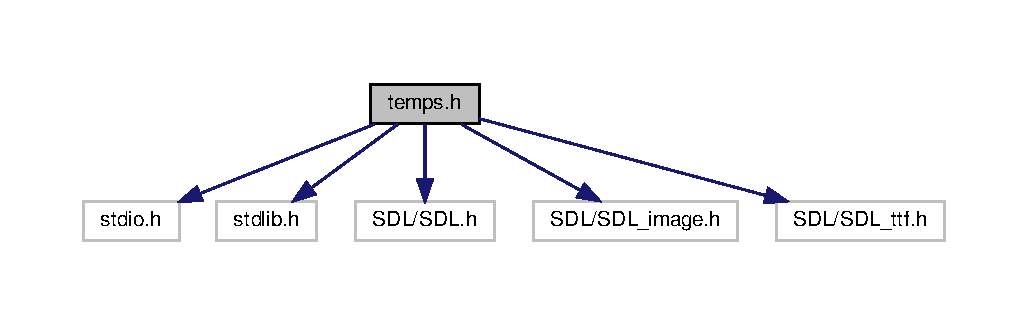
\includegraphics[width=350pt]{temps_8h__incl}
\end{center}
\end{figure}
This graph shows which files directly or indirectly include this file\+:
\nopagebreak
\begin{figure}[H]
\begin{center}
\leavevmode
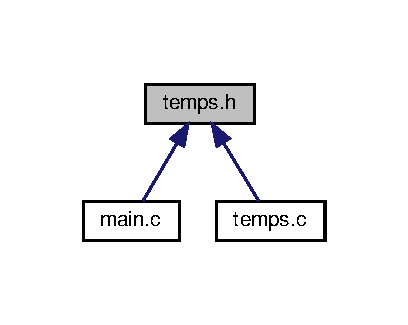
\includegraphics[width=196pt]{temps_8h__dep__incl}
\end{center}
\end{figure}
\subsection*{Data Structures}
\begin{DoxyCompactItemize}
\item 
struct \hyperlink{structtemps}{temps}
\begin{DoxyCompactList}\small\item\em struct for time \end{DoxyCompactList}\end{DoxyCompactItemize}
\subsection*{Functions}
\begin{DoxyCompactItemize}
\item 
\hyperlink{structtemps}{temps} \hyperlink{temps_8h_a8e74d45670becfd4b6a3718ea4a4543d}{inisaliser\+\_\+temp} (\hyperlink{structtemps}{temps} temp)
\begin{DoxyCompactList}\small\item\em To initialize the time . \end{DoxyCompactList}\end{DoxyCompactItemize}


\subsection{Function Documentation}
\mbox{\Hypertarget{temps_8h_a8e74d45670becfd4b6a3718ea4a4543d}\label{temps_8h_a8e74d45670becfd4b6a3718ea4a4543d}} 
\index{temps.\+h@{temps.\+h}!inisaliser\+\_\+temp@{inisaliser\+\_\+temp}}
\index{inisaliser\+\_\+temp@{inisaliser\+\_\+temp}!temps.\+h@{temps.\+h}}
\subsubsection{\texorpdfstring{inisaliser\+\_\+temp()}{inisaliser\_temp()}}
{\footnotesize\ttfamily \hyperlink{structtemps}{temps} inisaliser\+\_\+temp (\begin{DoxyParamCaption}\item[{\hyperlink{structtemps}{temps}}]{temp }\end{DoxyParamCaption})}



To initialize the time . 


\begin{DoxyParams}{Parameters}
{\em temp} & temps \\
\hline
\end{DoxyParams}
\begin{DoxyReturn}{Returns}
temp 
\end{DoxyReturn}

%--- End generated contents ---

% Index
\backmatter
\newpage
\phantomsection
\clearemptydoublepage
\addcontentsline{toc}{chapter}{Index}
\printindex

\end{document}
